\section{Coloring}

\frame{
{Part 2: Graph Isomorphism}

\tableofcontents[currentsection,hideallsubsections, firstsection=1, sections={1-4}]
}


\begin{frame}{Graph Coloring: Airplanes and boarding gates}

  Graph coloring is a problem with several applications, such as \structure{scheduling problems}. Let's look at Gate scheduling:\bigskip

    {\bf Example}:
    \begin{itemize}
    \item Every flight requires a \structure{gate} for embark/disembark;
    \item Sometimes flight times overlap, so multiple gates are necessary;
    \item How many gates do we need to satisfy a flight schedule?
    \end{itemize}

  \hfill 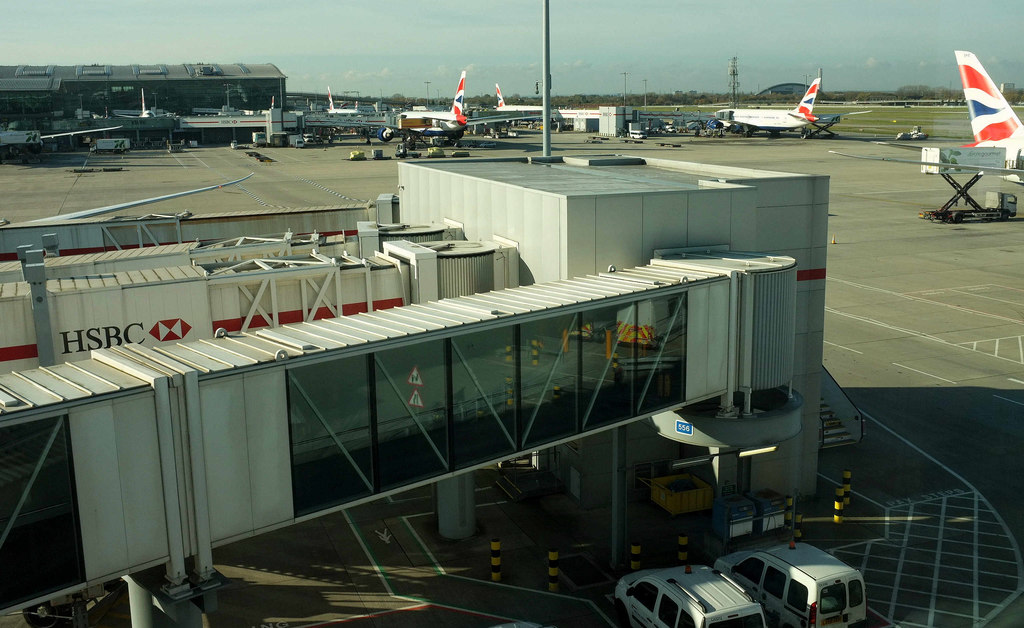
\includegraphics[width=0.5\textwidth]{../img/airgate}

\end{frame}

\begin{frame}{Boarding Gate Scheduling Graph}
  Let's define a \structure{Gate Scheduling Graph}, where each flight is a vertice, and an edge indicates that \alert{two flights are on the ground at the same time}.

    \begin{columns}[T]
      \column{0.6\textwidth}
      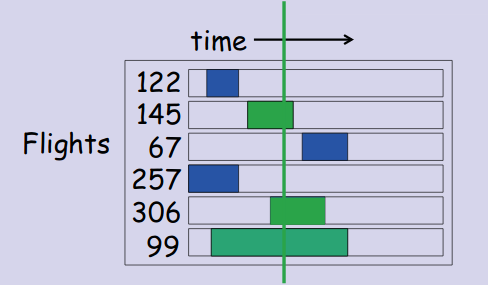
\includegraphics[width=1\textwidth]{../img/gatetable}
      \column{0.4\textwidth}
      \begin{tikzpicture}[scale=1.5,auto,swap]
        %\tikzset{edge/.style = {->,>=latex'}}
        \node[vertex] (a) at (0,3) {145};
        \node[vertex] (b) at (1,2) {309};
        \node[vertex] (c) at (0,0) {99};
        \draw[edge] (a) to (b);
        \draw[edge] (b) to (c);
        \draw[edge] (c) to (a);
      \end{tikzpicture}

    \end{columns}
\end{frame}

\begin{frame}{Gate Scheduling Graph and Coloring}
    \begin{columns}
      \column{0.5\textwidth}
      \begin{center}
      \begin{tikzpicture}[scale=1.5,auto,swap]
        %\tikzset{edge/.style = {->,>=latex'}}
        \node[vertex] (257) at (0,2) {257};
        \node[vertex] (122) at (1,2) {122};
        \node[vertex] (145) at (2,2) {145};
        \node[vertex] (306) at (0,0) {306};
        \node[vertex] (67) at (2,0) {67};
        \node[vertex] (99) at (1,-1) {99};
        \draw[edge] (257) to (122);
        \draw[edge] (257) to (99);
        \draw[edge] (122) to (99);
        \draw[edge] (306) to (99);
        \draw[edge] (67) to (99);
        \draw[edge] (306) to (67);
        \draw[edge] (306) to (145);
        \draw[edge] (145) to (99);
      \end{tikzpicture}
    \end{center}
      \column{0.5\textwidth}
      \begin{itemize}
        \item If each flight is a vertice, and each edge is a conflict, we can use \structure{graph coloring} to solve the problem.
        \item Each color is a new gate.
        \item If two vertices have an edge between them, the flights are \alert{in conflict}, and their colors must be different.
        \item The minimum number of colors to color all vertices is the same as the minimum number of boarding gates.
      \end{itemize}
    \end{columns}
\end{frame}


\begin{frame}{Gate Scheduling Graph and Coloring}
    \begin{columns}
      \column{0.5\textwidth}
      \begin{center}
      \begin{tikzpicture}[scale=1.5,auto,swap]
        %\tikzset{edge/.style = {->,>=latex'}}
        \node[red vertex] (257) at (0,2) {257};
        \node[blue vertex] (122) at (1,2) {122};
        \node[red vertex] (145) at (2,2) {145};
        \node[vertex] (306) at (0,0) {306};
        \node[blue vertex] (67) at (2,0) {67};
        \node[yellow vertex] (99) at (1,-1) {99};
        \draw[edge] (257) to (122);
        \draw[edge] (257) to (99);
        \draw[edge] (122) to (99);
        \draw[edge] (306) to (99);
        \draw[edge] (67) to (99);
        \draw[edge] (306) to (67);
        \draw[edge] (306) to (145);
        \draw[edge] (145) to (99);
      \end{tikzpicture}
    \end{center}
      \column{0.5\textwidth}
      \begin{itemize}
      \item We select colors for each vertex so that no adjacent
        vertex has the same color.

        \bigskip

      \item Each color = One new Gate

        \bigskip

      \item Final gate assignment:
        \begin{itemize}
        \item Blue Gate: Flight 122 and 67
        \item Red Gate: Flight 145 and 257
        \item Yellow Gate: Flight 99
        \item Gray Gate: Flight 306
        \end{itemize}

        \bigskip

      \item Can you find a better coloring using
        only \alert{3 gates}?
      \end{itemize}
    \end{columns}
\end{frame}

\begin{frame}{More Graph Coloring Problems}
    \begin{columns}
      \column{0.5\textwidth}
      \begin{itemize}
      \item \structure{Allocate classrooms} for courses.\\
        Some courses can be \alert{at the same time}.
        \medskip

      \item \structure{Allocate cages} for animals.
        Some animals \alert{can't live in the same cage}.
        \medskip

      \item \structure{Different Frequencies} for radio stations.
        Some frequencies \alert{interfere with each other}
        \medskip

      \item Color a map so that it look pretty!
      \end{itemize}

      \column{0.5\textwidth}
      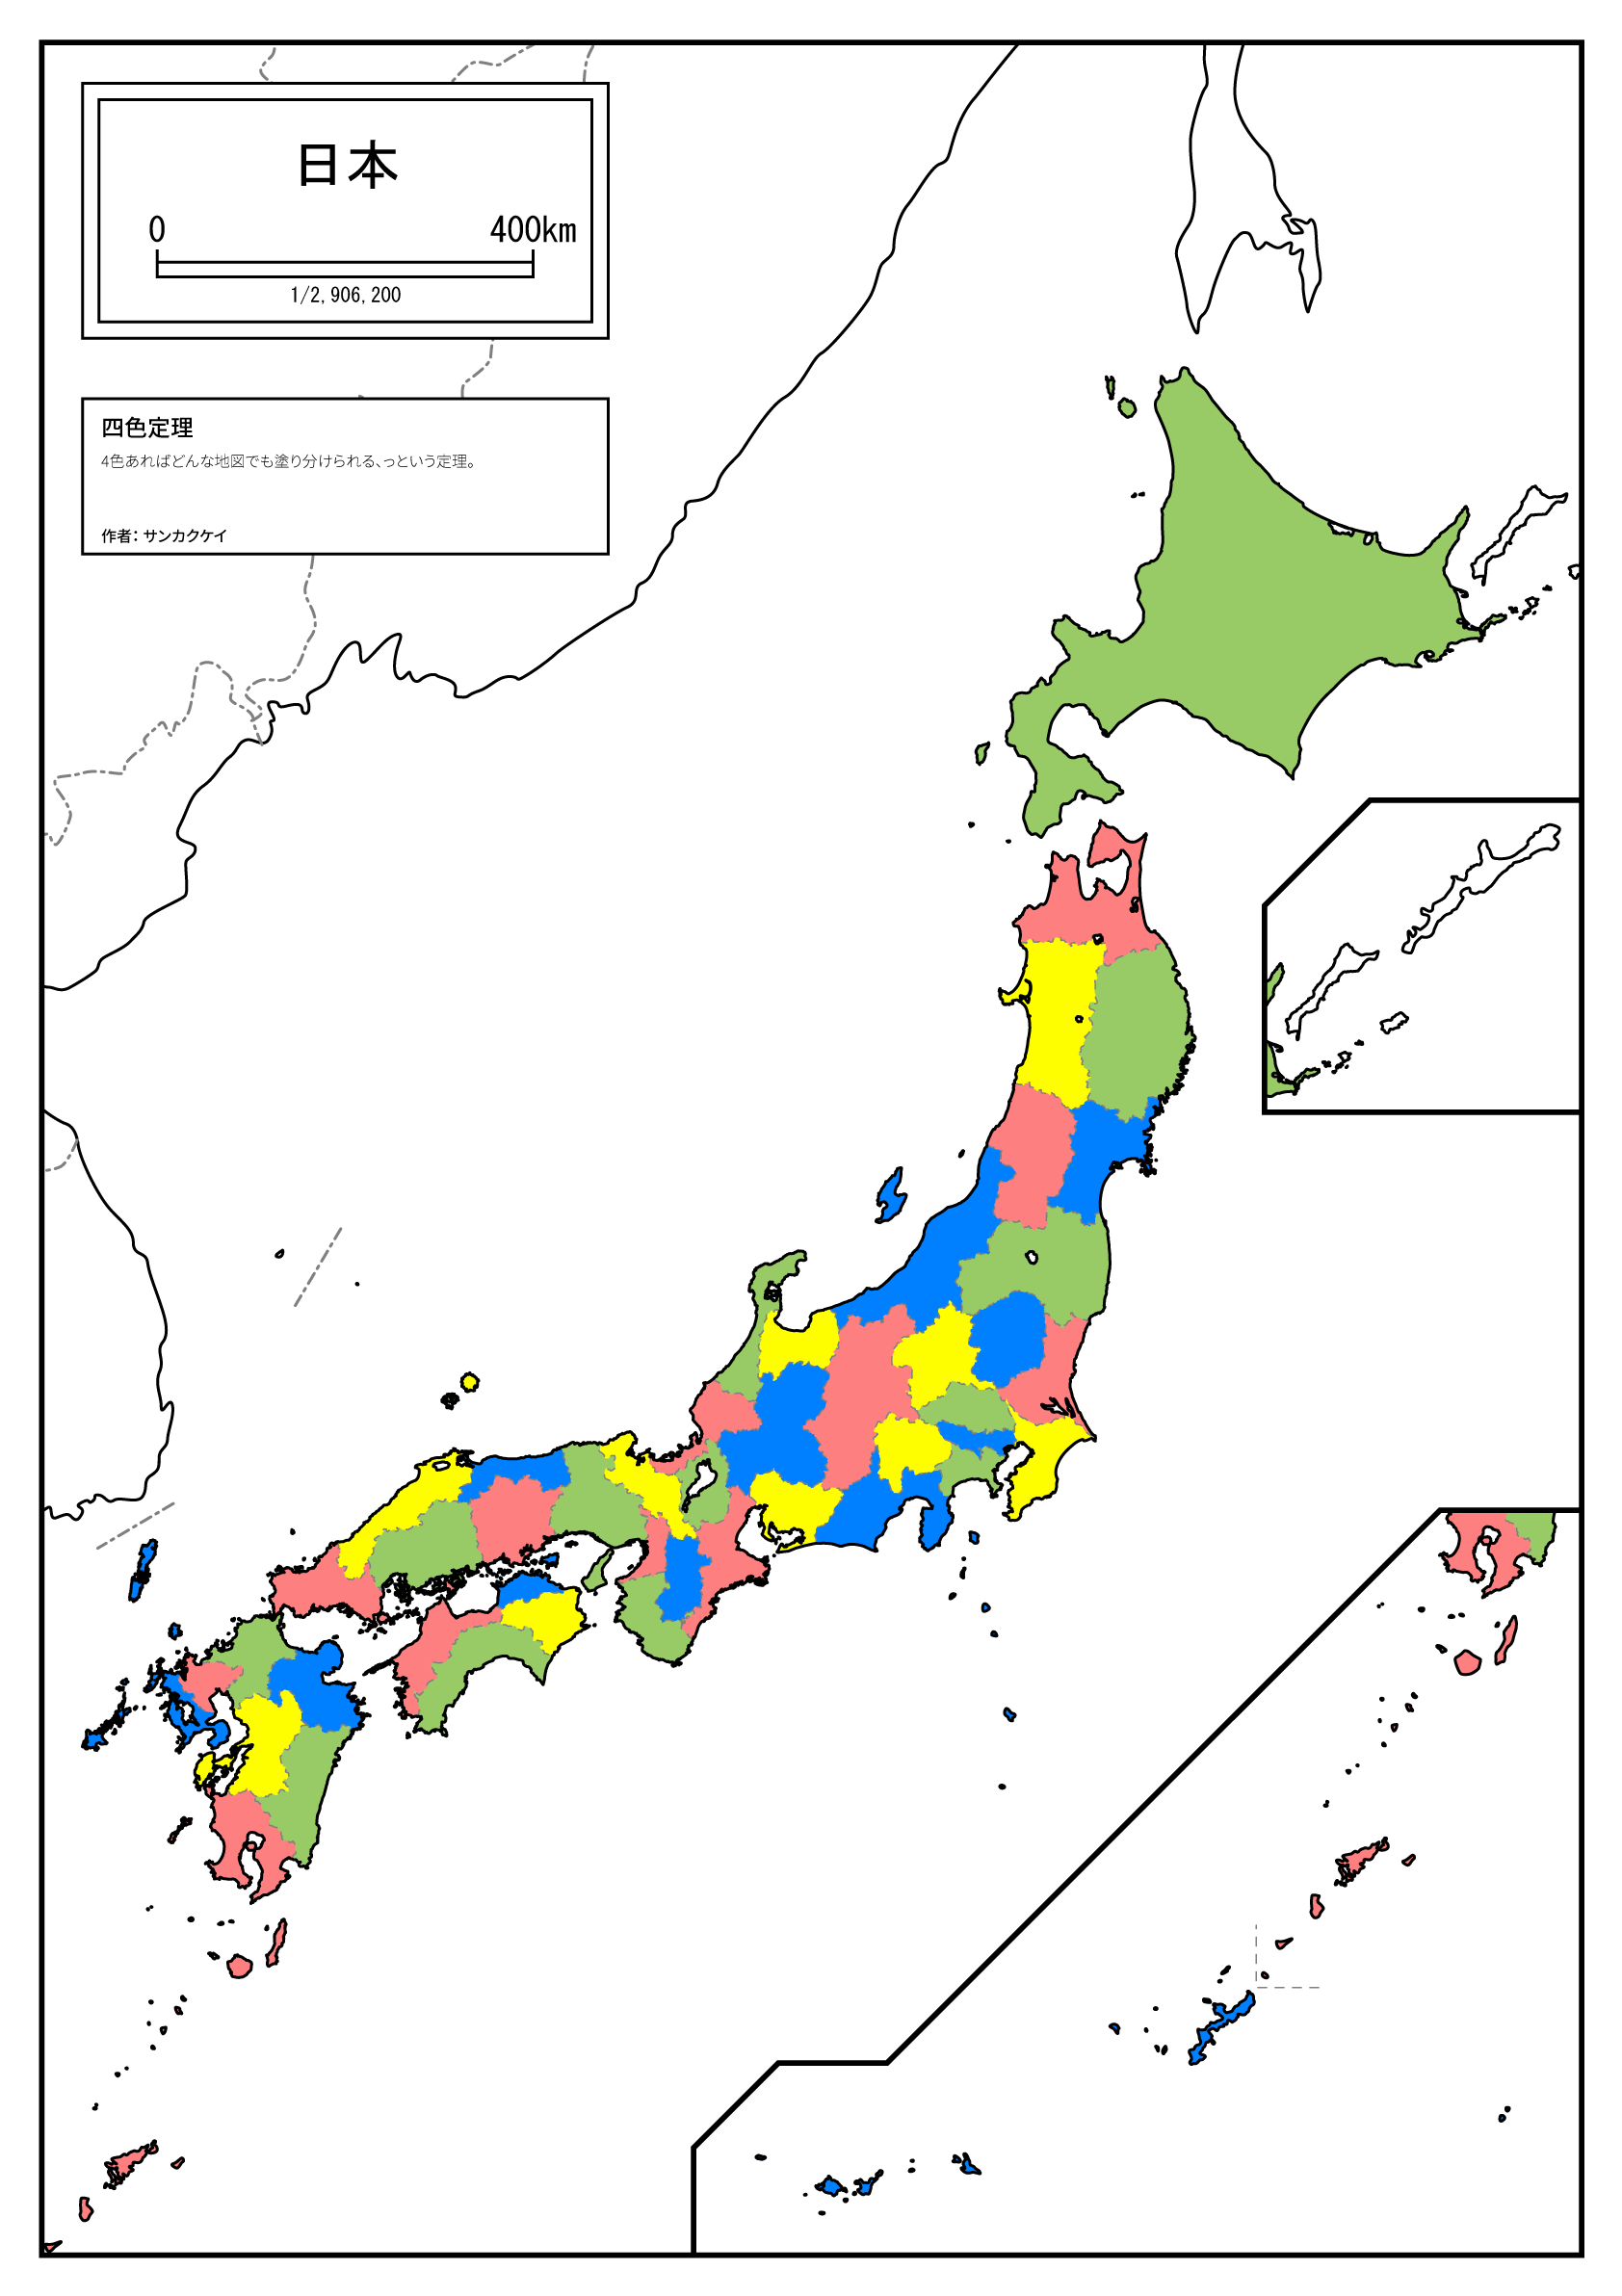
\includegraphics[height=.8\textheight]{../img/japan4color}
    \end{columns}
\end{frame}

\begin{frame}{Vertex Coloring and Face Coloring}

    \begin{center}
      Graphs (Vertices) to Maps (Faces) are equivalent when coloring!\\
      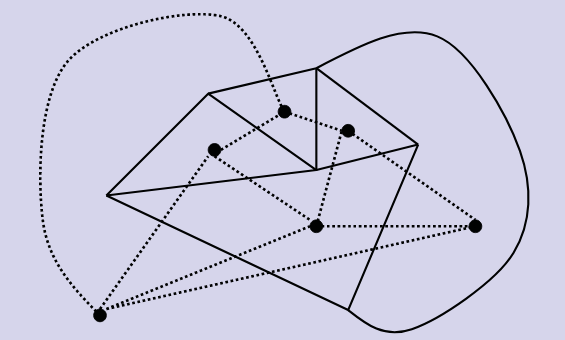
\includegraphics[width=0.5\textwidth]{../img/facecolor}
    \end{center}

    {\bf Theorem:} Maps can always be colored with 4 colors
    \begin{itemize}
    \item 1970: ``Proof'' with computers (automatically checks 1000's of maps)
    \item 1990: Better mathematical proof. (still needs programmed testing)
    \end{itemize}
\end{frame}

\begin{frame}{Chromatic Number}
    The Chromatic Number $\chi(G)$ is the \structure{minimum} number of
    colors needed for a graph $G$.

    {\bf Examples:} There are several rules for certain kinds of graphs:

    \begin{itemize}
    \item Cycle Graphs: $\chi(C_{\text{even}}) = 2$, $\chi(C_{\text{odd}}) = 3$\\
      \begin{tikzpicture}[scale=.8,auto,swap]
        %\tikzset{edge/.style = {->,>=latex'}}
        \node[red vertex] (a) at (0,0) {};
        \node[blue vertex] (b) at (1,0) {};
        \node[red vertex] (c) at (1,1) {};
        \node[blue vertex] (d) at (0,1) {};
        \draw[edge] (a) to (b);
        \draw[edge] (b) to (c);
        \draw[edge] (c) to (d);
        \draw[edge] (d) to (a);
        \node[red vertex] (a1) at (4,0) {};
        \node[blue vertex] (b1) at (5,0) {};
        \node[red vertex] (c1) at (5,1) {};
        \node[blue vertex] (d1) at (4,1) {};
        \node[yellow vertex] (e1) at (6,0) {};
        \draw[edge] (a1) to (b1);
        \draw[edge] (b1) to (e1);
        \draw[edge] (e1) to (c1);
        \draw[edge] (c1) to (d1);
        \draw[edge] (d1) to (a1);
      \end{tikzpicture}

    \item Complete Graph with $n$ vertices: $\chi(K_n) = n$\\
      \begin{tikzpicture}[scale=.8,auto,swap]
        %\tikzset{edge/.style = {->,>=latex'}}
        \node[red vertex] (a) at (0,0) {};
        \node[blue vertex] (b) at (1,0) {};
        \node[yellow vertex] (c) at (1,1) {};
        \node[vertex] (d) at (0,1) {};
        \draw[edge] (a) to (b);
        \draw[edge] (b) to (c);
        \draw[edge] (c) to (d);
        \draw[edge] (d) to (a);
        \draw[edge] (a) to (c);
        \draw[edge] (d) to (b);
      \end{tikzpicture}

    \item Wheel Graph: $\chi(W_{\text{odd}}) = 4, \chi(W_{\text{even}} = 3)$
      \begin{tikzpicture}[scale=.8,auto,swap]
        %\tikzset{edge/.style = {->,>=latex'}}
        \node[red vertex] (a) at (0,0) {};
        \node[blue vertex] (b) at (2,0) {};
        \node[red vertex] (c) at (2,2) {};
        \node[blue vertex] (d) at (0,2) {};
        \node[yellow vertex] (e) at (1,1) {};
        \draw[edge] (a) to (b);
        \draw[edge] (b) to (c);
        \draw[edge] (c) to (d);
        \draw[edge] (d) to (a);
        \draw[edge] (a) to (e);
        \draw[edge] (b) to (e);
        \draw[edge] (c) to (e);
        \draw[edge] (d) to (e);
      \end{tikzpicture}
    \end{itemize}
\end{frame}

\begin{frame}{Bounding Chromatic Numbers}{What is the maximum Chromatic Number?}

    \begin{itemize}
    \item If all vertex degrees are $\leq k \implies \chi(G) \leq k+1$\\
      \hfill (Proof by Greedy coloring algorithm).

      \bigskip

    \item Is a graph 2-colorable?\\
      \hfill ({\bf easy} to check: do a Breath First Search and mark as you go)\bigskip

    \item Is a graph 3-colorable?\\
      \hfill ({\bf very hard} to check: NP complete!)\bigskip

    \item Is $\chi(G) = k$?\\
      \hfill (in theory not harder than 3 color, harder in practice).

    \end{itemize}
\end{frame}

\subsection{Connectivity}

\begin{frame}{Connectivity}{Definition}

    \begin{itemize}
    \item Two vertices are \structure{connected} {\bf iff} there is a \structure{path} between the two.\bigskip

    \item Every vertice is connected to itself. (even if it does not have a self-edge)\bigskip

    \item A whole \structure{graph} is \structure{connected} if every vertice is connected to each other.
    \end{itemize}\bigskip

    \begin{center}
      \begin{tikzpicture}[scale=.8,auto,swap]
        %\tikzset{edge/.style = {->,>=latex'}}
        \node[vertex] (a) at (0,0) {a};
        \node[vertex] (b) at (2,0) {b};
        \node[vertex] (c) at (2,2) {c};
        \node[vertex] (d) at (0,2) {d};
        \node[vertex] (e) at (1,1) {e};
        \node[vertex] (f) at (3,0) {f};
        \node[vertex] (g) at (4,2) {g};
        \draw[edge] (a) to (b);
        \draw[edge] (b) to (c);
        \draw[edge] (c) to (d);
        \draw[edge] (d) to (a);
        \draw[edge] (a) to (e);
        \draw[edge] (b) to (e);
        \draw[edge] (c) to (e);
        \draw[edge] (d) to (e);
        \draw[edge] (f) to (g);
      \end{tikzpicture}
    \end{center}
\end{frame}

\begin{frame}{Connected Components}{Vertex Connectivity}

    \begin{center}
      \begin{tikzpicture}[scale=.8,auto,swap]
        %\tikzset{edge/.style = {->,>=latex'}}
        \node[vertex] (a) at (0,0) {a};
        \node[vertex] (b) at (2,0) {b};
        \node[vertex] (c) at (2,2) {c};
        \node[vertex] (d) at (0,2) {d};
        \node[vertex] (e) at (1,1) {e};
        \node[vertex] (f) at (4,0) {f};
        \node[vertex] (g) at (5,2) {g};
        \node[vertex] (h) at (3,1) {h};
        \draw[edge] (a) to (b);
        \draw[edge] (b) to (c);
        \draw[edge] (c) to (d);
        \draw[edge] (d) to (a);
        \draw[edge] (a) to (e);
        \draw[edge] (b) to (e);
        \draw[edge] (c) to (e);
        \draw[edge] (d) to (e);
        \draw[edge] (f) to (g);
      \end{tikzpicture}
    \end{center}

    \begin{itemize}
    \item Every Graph is composed of connected subgraphs called
      \structure{connected~components}
    \item \structure{connected component} of
      v $::=$ \{w | w connected to v\}.
    \item \structure{connected component} of $v = E^*(v)$
      (walk relation of v)

      \bigskip

    \item A graph is \structure{connected} {\bf iff} it has exactly 1 connected component.
    \end{itemize}
\end{frame}

\begin{frame}{Connected Components}{Edge connectivity}

    \begin{itemize}
    \item vertices $v,w$ are \structure{k-edge} connected if
      they remain connected \alert{even if fewer than $k$ are deleted}.

      \begin{center}
      \begin{tikzpicture}[scale=.8,auto,swap]
        %\tikzset{edge/.style = {->,>=latex'}}
        \node[vertex] (a) at (0,0) {a};
        \node[red vertex] (b) at (2,0) {b};
        \node[blue vertex] (c) at (2,2) {c};
        \node[blue vertex] (d) at (0,2) {d};
        \node[vertex] (e) at (1,1) {e};
        \node[vertex] (f) at (4,0) {f};
        \node[red vertex] (g) at (5,2) {g};
        \node[vertex] (h) at (3,1) {h};
        \draw[edge] (a) to (b);
        \draw[edge] (b) to (c);
        \draw[edge] (c) to (d);
        \draw[edge] (d) to (a);
        \draw[edge] (a) to (e);
        \draw[edge] (b) to (e);
        \draw[edge] (c) to (e);
        \draw[edge] (d) to (e);
        \draw[edge] (f) to (g);
        \draw[edge] (f) to (h);
        \draw[edge] (g) to (h);
        \draw[edge] (h) to (b);
      \end{tikzpicture}
    \end{center}

    \item In this graph, the \structure{blue vertices} are 3-edge connected, and the \alert{red vertices} are 1-edge connected;
    \item A {\bf Graph} is k-edge connected if all pairs of vertices are \structure{at least} k-edge connected.
    \end{itemize}
\end{frame}

\begin{frame}{Connected Components}{Edge Connectivity}

  {\large

    \begin{itemize}

    \item {\bf Edge Connectivity} represents the degree of
      {\bf fault tolerance} in a graph.


    \item {\bf Example:} In a communication network, how many
      channels can fail before communication is disrupted?

      \bigskip

    \item Related Concept: \structure{k-vertice connectivity}

      \begin{itemize}
      \item k-vertice connected graph $\implies$ k-edge connected;
      \item \alert{BUT!} k-edge connected $\not\implies$ k-vertice
        connected.
      \end{itemize}

    \item The \structure{complete graph} $K_n$ is n-1 connected.
    \end{itemize}
  }

\end{frame}

\begin{frame}
  \frametitle{Connectivity and Hypercubes}

  {\larger

      \begin{center}
      \begin{tikzpicture}[scale=.8,auto,swap]
        %\tikzset{edge/.style = {->,>=latex'}}
        \node[vertex] (00) at (0,0) {00};
        \node[vertex] (01) at (-2,0) {01};
        \node[vertex] (10) at (0,2) {10};
        \node[vertex] (11) at (-2,2) {11};
        \draw[edge] (00) to (10);
        \draw[edge] (10) to (11);
        \draw[edge] (00) to (01);
        \draw[edge] (01) to (11);

        \node[vertex] (000) at (3,0) {000};
        \node[vertex] (010) at (5,0) {010};
        \node[vertex] (100) at (3,2) {100};
        \node[vertex] (110) at (5,2) {110};
        \node[vertex] (001) at (4,1) {001};
        \node[vertex] (011) at (6,1) {011};
        \node[vertex] (101) at (4,3) {101};
        \node[vertex] (111) at (6,3) {111};
        \draw[edge] (000) to (100);
        \draw[edge] (100) to (110);
        \draw[edge] (000) to (010);
        \draw[edge] (010) to (110);
        \draw[edge] (001) to (101);
        \draw[edge] (101) to (111);
        \draw[edge] (001) to (011);
        \draw[edge] (011) to (111);
        \draw[edge] (001) to (000);
        \draw[edge] (111) to (110);
        \draw[edge] (011) to (010);
        \draw[edge] (101) to (100);


      \end{tikzpicture}
    \end{center}

    \begin{itemize}
    \item Consider the $n$-dimensional hypercube $H_n$
    \item $V(H_n) ::= \{0,1\}^n$
    \item $E(H_n) ::= \{(u,v)$ {\bf iff} u and v differ in 1 bit $\}$

    \item $H_n$ is $n$ vertex connected. ($H_n$ has $n^2$ vertices)
    \end{itemize}

  }

\end{frame}
